%%%%%%%%%%%%%%%%%%%%%%%%%%%%%%%%%%%%%%%%%%%%%%%%%%%%%%%%%%%%%%%%%%
%%%%%%%% ICML 2013 EXAMPLE LATEX SUBMISSION FILE %%%%%%%%%%%%%%%%%
%%%%%%%%%%%%%%%%%%%%%%%%%%%%%%%%%%%%%%%%%%%%%%%%%%%%%%%%%%%%%%%%%%

% Use the following line _only_ if you're still using LaTeX 2.09.
%\documentstyle[icml2013,epsf,natbib]{article}
% If you rely on Latex2e packages, like most moden people use this:
\documentclass{article}

% For figures
\usepackage{graphicx} % more modern
%\usepackage{epsfig} % less modern
\usepackage{subfigure} 

% For citations
\usepackage{natbib}

% For algorithms
\usepackage{algorithm}
\usepackage{algorithmic}

% As of 2011, we use the hyperref package to produce hyperlinks in the
% resulting PDF.  If this breaks your system, please commend out the
% following usepackage line and replace \usepackage{icml2013} with
% \usepackage[nohyperref]{icml2013} above.
\usepackage{hyperref}

% Packages hyperref and algorithmic misbehave sometimes.  We can fix
% this with the following command.
\newcommand{\theHalgorithm}{\arabic{algorithm}}

% Employ the following version of the ``usepackage'' statement for
% submitting the draft version of the paper for review.  This will set
% the note in the first column to ``Under review.  Do not distribute.''
%\usepackage{icml2013} 
% Employ this version of the ``usepackage'' statement after the paper has
% been accepted, when creating the final version.  This will set the
% note in the first column to ``Proceedings of the...''
\usepackage[accepted]{icml2013}


% The \icmltitle you define below is probably too long as a header.
% Therefore, a short form for the running title is supplied here:
\icmltitlerunning{Submission and Formatting Instructions for ICML 2013}

\begin{document} 

\twocolumn[
\icmltitle{Twitter Trend Detection and Classification}

% It is OKAY to include author information, even for blind
% submissions: the style file will automatically remove it for you
% unless you've provided the [accepted] option to the icml2013
% package.
\icmlauthor{Fei Xie}{virgilxie@gmail.com}
\icmladdress{Carnegie Mellon University,
            5000 Forbes Ave, Pittsburgh, PA 15213 USA}
\icmlauthor{Pengqi Liu}{lpq1990@gmail.com}
\icmladdress{Carnegie Mellon University,
            5000 Forbes Ave, Pittsburgh, PA 15213 USA}
\icmlauthor{Zeyuan Li}{zeyuanl@cmu.edu}
\icmladdress{Carnegie Mellon University,
            5000 Forbes Ave, Pittsburgh, PA 15213 USA}          

% You may provide any keywords that you 
% find helpful for describing your paper; these are used to populate 
% the "keywords" metadata in the PDF but will not be shown in the document
\icmlkeywords{boring formatting information, machine learning, ICML}

\vskip 0.3in
]

\begin{abstract} 
%Detecting Twitter Trend has great applicant values in real world, such as promoting political policies, avoiding rumors' transmission, etc.. Thus understanding the twitter trend patterns is very important. In this paper, we implemented several different methods including both content-based and time-series algorithm on classifying trend patterns. By doing experiments on large streaming twitter data, we discussed their effectiveness in achieving our goals.
Detecting Twitter Trend has great applicant values in real world, such as promoting political policies, avoiding rumors' transmission, etc.. Thus understanding the twitter trend patterns is very important. In this paper, we implemented several different methods including both content-based and time-series-based algorithm to classify trend patterns. By doing experiments on a large set of twitter data, we can finally predict the trend pattern with F-measure $0.57$, which is nearly $200\%$ better than the baseline methods.
\end{abstract} 

\section{Introduction}
In recent years, social network is becoming more and more popular, which brings up an explosion in the research of social media data. Lots of valuable information is hidden in the large quantity of data. Machine learning in large scale technology made it easier to exploit underlying information in the huge data.

In this paper, we study the problem of prediction trend type using large amounts of data. Specifically, we try to predict the possible future trend pattern of an emerging topic, analyze trend and understand what's going on at Twitter more accurately. In the first part, we study on content and temporal information cooperated with different kinds of machine learning method to predict the trend type of information. Then we experiment with the combination of features and methods. Result and conclusion is given at last.
\label{submission}



\section{Related Work} 
The paper \cite{nikolov2012trend} introduced a new approach to detect Twitter trends in a nonparametric method. It presented a general time series analysis method that can be used to detect the future trend on twitter. This paper used both positive trending examples and negative, or non-trending example to vote for the current observation sequence. Then based on the voting result to find out whether it's a trend or not. The result of this paper is fairly good. In 79\% percent of cases, this paper detected trending topics earlier than Twitter (1.43 hours earlier), and it managed to keep an error rate of around 95\% (4\% false positive rate, 95\% true positive rate). As this paper's experiment result shows that it is fairly good to use time series data to predict trends in twitter, we believe the time series prior of the peak would be a good indictor of the trend pattern.
 
The paper \cite{journals/corr/abs-1102-1402} made a detail analysis on different kinds of factors that may affect the persistence and decay of twitter trend based on history data and experiments. It showed that the resonance of the content with the users of the social network plays a major role in causing trends.It also demonstrate empirically how factors such
as user activity and number of followers do not contribute strongly to trend creation and its propagation. Based on the conclusion of this paper, we believe that content of twitter activity has a major influence to the type of twitter trends.

There is also a line of work about time series clustering. The paper \cite{Yang11} studied how the trend pattern of confine content's popularity grow and fade over time. In order to do that, the paper introduced a new K-SC algorithm, which is essentially the K-means algorithm but using different similarity metrics as well as using a different way to compute the cluster center.  They tested on a set of tweets and a set of blogs and news articles. They finally showed there were six major patterns in online content.  

\section{Dataset} 

We extract nearly 200 million tweets from Brendan's ``Gardenhose" archive from June 2009 to February 2010 as same time period as described in the paper \cite{Yang11}. And we further extract 2.5 million all the tweets containing the top 998 most frequently appeared hashtags. This data size is about 600MB compressed and $>$3GB uncompressed.  

Besides that, we also build our time series based on the number of tweets in each one hour unit. For the known peak time series, we build time series using the truncated time series of 128 hours with peak located at the 1/3 of the 128 hours. For the unknown peak time series, we build time series throughout the whole eight months. 

\section{Method}

Twitter trends are measured by the activity of Twitter hashtags or topics. In our work, we use the activity of hashtag to measure Twitter trend. We want to predict the future trend of an emerging hashtag/topic based on either content or some previous temporal information from tweets containing that hashtag. For example, we want to predict future trend of hashtag ``\#protest" based on some previous tweets containing that hashtag, like \texttt{"RT Iranian women must liberate themselves http://rurl.org/1rlv \#protest \#nytimes"}.

The problem can be approached as a supervised learning problem. We first assign each hashtag a trending pattern based on its time series. Although this problem is a supervised learning problem, we label the instances through clustering. From then on, we can train a classifier based on either text content or time series from hashtag histogram. And we could then classify the hashtag to different patterns using our classifier. 

The content and temporal information maybe beneficial in predicting the trend pattern of a hashtag. We use content information because some words or phrases reveal their trend to some extent. For example, the trend pattern of ``\#olympics" is different from ``\#apple" that ``\#olympics" is reoccurring every four years and it will only be a trend when it is going on, while ``\#apple" is a daily trend and can trigger a trend very often like it has new product to release or new dispute with competitors. The context words associate with ``\#olympics", like athlete names ``Michael Phelps" and medals "Gold Medal", and ``\#apple", like product name ``iPhone" and competitor name "Samsung", are quite informative when training and testing using classifiers. We also use temporal information like the time series (histogram volume) as an another way to predict trend. The ups and downs in different time series can also indicate different patterns.      

In our paper, we have used K-SC algorithm to do Trend Clustering of time series \cite{Yang11}. We have tried four different approaches to do Trend Prediction.  

\subsection{Trend Clustering}

We do Trend Clustering mainly to label the data, which assign a label to a time series according to which cluster it belongs. We use these labeled data to do training and testing on our classifiers. 

We use the K-SC algorithm \cite{Yang11} to do clustering of the 128 hours time series with peak located at 1/3 of the 128 hours. This algorithm is very similar to K-means algorithm. It has for each data points calculate which nearest cluster centroid it belongs and then compute the new cluster centroid again. The only two differences with K-means are K-SC uses the special designed similarity metric, which is similar to Time Wrapping Distance (compute distance after shifting and scaling). Another difference is K-SC uses a new method to compute cluster centroid, which is essentially select the centroid that minimize the squared distance over all data points to their closest centroid using the new similarity metric.     

We choose to K=6 and the clustering result in Figure~\ref{six-cluster}

\begin{figure}[ht]
\vskip 0.2in
\begin{center}
\centerline{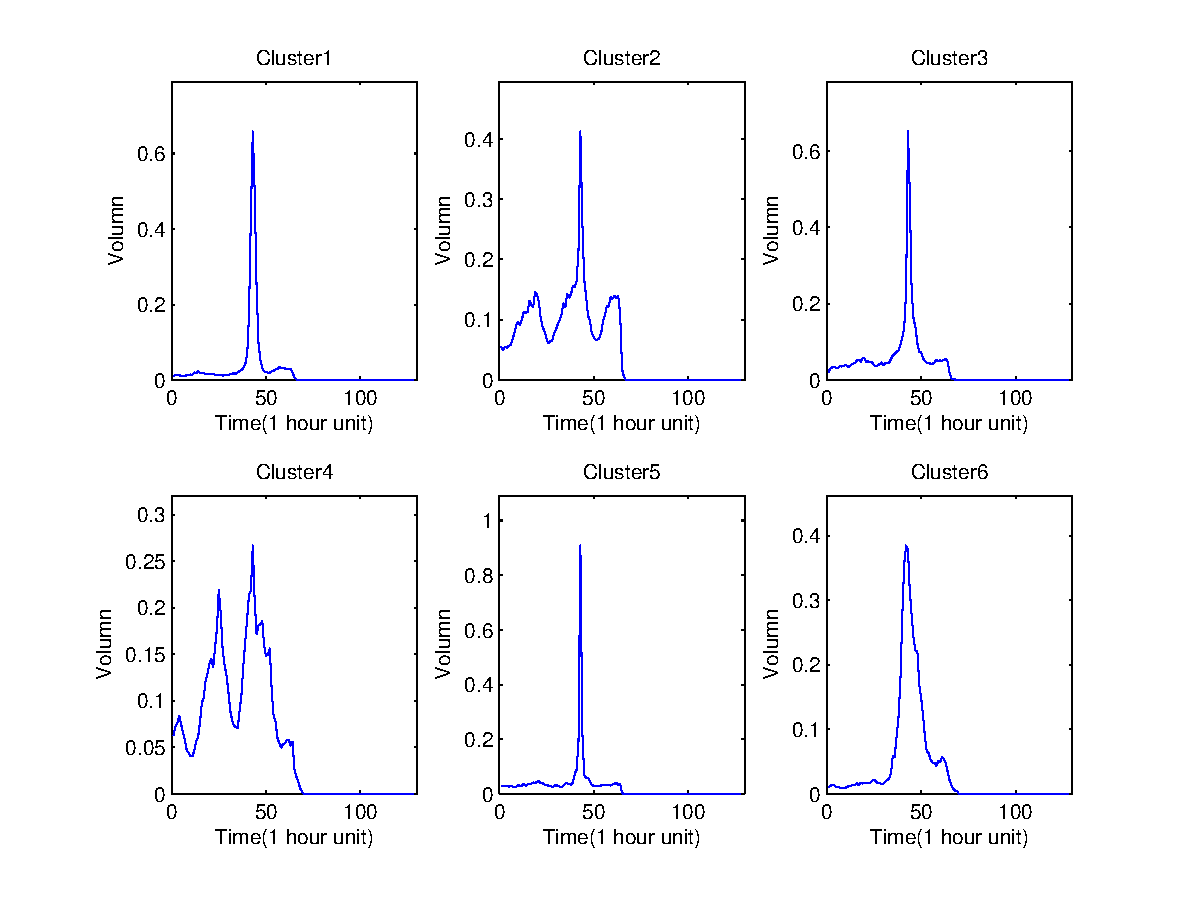
\includegraphics[width=\columnwidth]{sixClusters}}
\caption{All model performance using different metrics.}
\label{six-cluster}
\end{center}
\vskip -0.2in
\end{figure} 

\subsection{Trend Prediction}

For predicting Twitter trend, we can consider using both content information and temporal information as the clue for the trending activity.   

\subsubsection{Bag-of-Word Naive Bayes Trend Prediction}
The Naive Bayes Method is the first one we come up with in this project. Since this is a classification problem and tweets are composed of words and tokens, the use of bag of word model is very intuitive. The Naive Bayes algorithm we implemented is similar to the one we did in homework. For the training set, each tweet has a label (1 to 6), so each of them can be treated as a training sample. We first utilize LingPipe to tokenize the tweets by considering lowercase, stemming, etc. Then with these separate tokens, we count the number of co-occurrence and other metrics needed to build the Naive Bayes model. The whole process was done very quickly and efficiently using Hadoop.
After getting all the model parameters we need, we start working on the test data. The log likelihood of each test sample can be written as:
\begin{equation} 
(\prod_{j=1}^d  \frac{C(X_j=x_j \wedge Y=y')+mq_j}{C(Y=y')+m})\frac{C(Y=y')+mq_j}{C(Y=ANY)+m}
\end{equation}
Using this equation, we can easily classify our test tweets data into one of the six categories. But here we made some changes on the test process. We first combine several tweets of the same hashtag into one document, then apply the NB classifiers. The reason we did so is because the tweets are often very short, thus making the token distribution very sparse which may lead to bad result. 

In addition to this traditional Naive Bayes method, we also take the weight of token into account. We believe that some of the words must be more important than others when apply to certain situations or categories. For example, people won't talk about Hurricane too often usually, but when we have a real Hurricane in the world, the world Hurricane becomes important. To discover such important tokens and give different weight on them, we first calculate both background and foreground token distributions, and use Chi-square method to find those important words. The Chi-Square method can be written as

\begin{equation} 
\frac{(fg-bg)^2}{bg}
\end{equation}

By using this model, we successfully find out those important words give certain cluster. For example, in cluster 3, the top 10 words include mac, apple, ipad, ipod, chrome, android, etc., which are all relevant to IT fields. Though this token weight makes sense, when apply to Naive Bayes Model, we didn't find good improvement on the final results. Maybe our combine method is not good enough, which we may dig deeper later.

\subsubsection{Bag-of-Word Logistic Regression Trend Prediction}

In trend prediction using bag-of-word Logistic Regression, we treat all words in the tweets containing the hashtag as a document (bag-of-word). The document's label is the hashtag's label assigned in Trend Clustering part based on the clustering result from hashtag's time series. For this specific Logistic Regression problem, we want to maximize log likelihood $L(w)=\Pi_lP(y^l|x^l,w)$, where $x^l$ represents the $l$th training document (BOW of all words in tweets containing the same hashtag), $y^l$ represents the class label of $l$th training document and $w$ is the model weight. Using stochastic gradient descent, we can derive the training rules as 

\begin{equation} 
w_{ij}=w_{ij} + \lambda(y^l - \hat{y}^l) x^l - 2\lambda \mu w_{ij} \label{eq:lrtrain}
\end{equation}

where $w_{ij}$ is the $i$th classifier's $j$th element in weight vector, $y^l$ is the true class label of $l$th training document, $\hat{y}^l$ is the predicted probability of chewing this label as the class label of $l$th training document, $x^l$ is the bag-of-words in $l$th training document,  $\lambda$ is the gradient step size, $\mu$ is the regularization constant. To make our algorithm more fast and space efficient for processing large data, we use the delayed update stochastic gradient descend with hash trick that introduced in class. 

Since this specific Logistic Regression classifier is a multi class classifier, we train multiple binary classifier and choose the label with the largest weight in the test phase. The testing document consists of bag-of-words all words in tweets containing the same hashtag. The test rules is    

\begin{equation} 
y^l =\arg\max_i  \sum_j w_{ij} x_j^l\label{eq:lrtest}
\end{equation}

where $w_{ij}$ is the $i$th classifier's $j$th element in weight vector, $y^l$ is the predicted class label for $l$th testing instance, $x_j^l$ is the $j$th word (feature after hash trick) in $l$th testing document. 

\subsubsection{Time Series Similarity Measurement}
After working on content based measurement of  Twitter trend, we turn to use temporal information with hashtag to classify and predict the type of Twitter trend. Based on the former research\cite{nikolov2012trend} about the twitter trend,
we believe time series prior of the peak would be a good indictor of the trend pattern. So we add this part time series information to do classification and prediction.
Different from \cite{nikolov2012trend}, we not only need to predict if the sequence of tweets will be a trend, but also decide which trend pattern it would be. The meaning of doing this is find the spread pattern of twitter trend before the trend reaches its peak.  Because of time limitation, we applied a parametric model to predict and classify the trend pattern instead of using a nonparametric prediction. The whole process could be divided into two steps. Trend prediction and Trend classification.

The trend prediction is find the twitter activity that could become a trend. We can assume that a normal trend model of tweet activity is roughly constant with occasional jumps. So the detection process is similar with a filter, which is used to filter the occasional jump and find the true jump that become a twitter trend.

Here we define a trend by two variables, jump rate and popularity duration. Jump rate is 
\begin{equation} 
\frac{\alpha * standard variance}{mean}
\end{equation}
The standard variance and mean refer to the twitter activity of the according time interval.
Popularity duration is the total volume in a time interval. If the popularity duration is beta times higher than the mean popularity duration value. We will consider this is a trend. As this is a parametric model, alpha and beta needs to be estimated by experiment. When monitoring the twitter activity, we use a sliding window to check if current trend would become a twitter trend. A acceleration step applied here that we don't need to compute the parametric model every hour but only when the twitter activity has a large increase. 
The above detection process is illustrated in Figure~\ref{imgjump}.
\begin{figure}[ht]
\vskip 0.2in
\begin{center}
\centerline{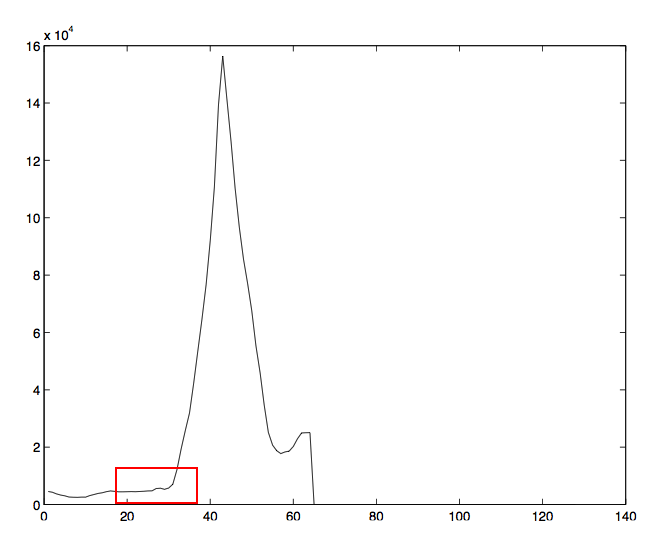
\includegraphics[width=\columnwidth]{jump}}
\caption{The detection of a big jump}
\label{imgjump}
\end{center}
\vskip -0.2in
\end{figure} 
When the sliding window comes  to a beginning of trend, we can see in the red box, the jump rate and popularity duration is satisfied by the parametric model. We will consider this is a big jump, which imply the follow twitter activity will become a trend. Then we will come to the classification step to decide the type of the possible trend.

In the above step, we already get the trend patterns. So we apply a similarity measurement to classify the pattern of possible trend. As this twitter time series activity is discrete data, we compute the similarity of current twitter activity to each patterns for each hour. In another words, each hour in the time interval will vote for each trend pattern based on similarity between the instance in detected time interval and trend patterns.
The similarity is defined by a decaying exponential, in this form, the nearest time series data has more weights while the non-similar data has less weight. Similarity defined as follows:
\begin{equation} 
Similarity(instance, pattern) = e^{-d(i, p)}
\end{equation}
In the above equation, i means the time series data at time i. p means the detected pattern time series data in the according time i. d(i, p) is the euclidean distance between i and p. The similarity measurement process is illustrated in figure ~\ref{imgcmp}
\begin{figure}[ht]
\vskip 0.2in
\begin{center}
\centerline{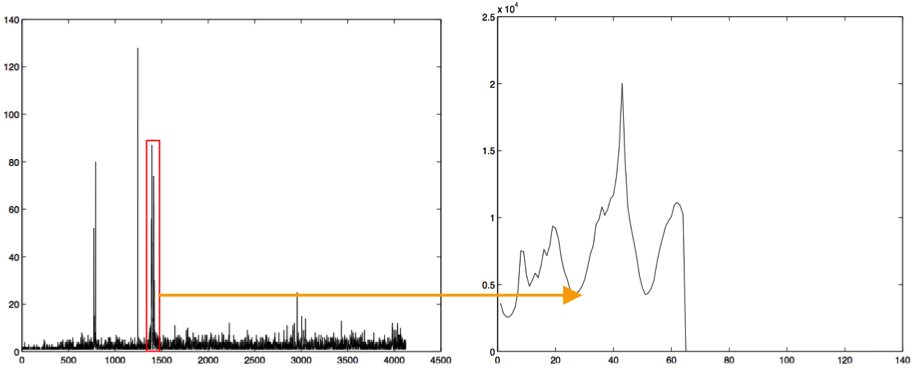
\includegraphics[width=\columnwidth]{compare}}
\caption{Illustration of similarity measurement process}
\label{imgcmp}
\end{center}
\vskip -0.2in
\end{figure} 
The left subfigure in figure~\ref{imgcmp} is a section of twitter activity of certain hashtag, which is the time series data of 8 month. We can see that there could be several small jumps leading up to a big jump. The right subfigure in figure~\ref{imgcmp} is a detected pattern of twitter trend, which is the time series data of 128 hours of all twitter activity in this pattern.  


\subsubsection{Time Series Logistic Regression Trend Prediction}

Although bag-of-words model can give us some hints about future trend, using content information to predict temporal pattern is somewhat limited. Because words alone are not always correlated with trend. Therefore, we use directly a time interval in time series (hashtag histogram) to predict the future trend pattern. 

Since we have clustered the time series using the 128 hours time series, placing the peak at one third in the whole 128 hours time series, we assume that the time interval prior to a trend (0-43 hour) is a good indicator of future pattern of trend. We define trend as a sudden jump in the time series here. Therefore, we still model the problem as a classification problem that we can train and test using Logistic Regression based on the data points in a short interval that in the very beginning of time series. 

We always choose the interval prior to a trend (sudden jump in time series) to train and test, since we want to predict the future pattern of trend as quickly as possible with least amount of previous known data. Therefore, the problem becomes to detect trend and use the interval of time series when the trend just begin gaining popularity to train and test our classifier. We can then try to solve the transformed problems with two assumptions here: predict trend patterns with known trend and predict trend patterns with unknown trend. 

{\bf Predict Trend Patterns with Known Trend:} We use the only trend that leads to peak (sudden jump in highest time series globally) in time series as the best trend as the interval for training and testing. With known most salient trend, we could get more good training instances and thus good classifier which leads to better testing results.

{\bf Predict Trend Patterns with Unknown Trend:} We now need to detect a relative good trend (sudden jump in highest time series locally) by our trend detection algorithm. The detection algorithm needs to find real potential trend instead of small fluctuations. The algorithm is parametric that it needs parameter tuning to avoid this. 






\section{Experiment} 

\subsection{Content (BOW) vs Temporal (Time Series)}

We can see from Table~\ref{tab-result} the final evaluation result from the table below. Note that ``BOW\_NB" and ``BOW\_LR" represents Naive Bayes and Logistic Regression using Bag-of-Word model respectively. ``TS\_LR\_KT" and ``TS\_LR\_UNKT" represents Logistic Regression with known trend and unknown trend using time series model respectively. The time series model only have trained and tested using only a interval of nine data points (first nine hours of a trend which the popularity is about to go up).  

\begin{table}[t]
\caption{Model performance using different metrics}
\label{tab-result}
\vskip 0.15in
\begin{center}
\begin{small}
\begin{sc}
\begin{tabular}{lcccr}
\hline
\abovespace\belowspace
Model Name & Precision & Recall & F-measure \\
\hline
\abovespace
BOW\_NB   & 0.22 & 0.22 & 0.22 \\		
BOW\_LR & 0.34 & 0.13 & 0.19 \\		
TS\_LR\_KT    & \textbf{0.57} & \textbf{0.57} & \textbf{0.57} \\	
TS\_LR\_UNKT   & 0.31 & 0.34 & 0.33     \\
TS\_SM\_UNKT	& 0.19	& 0.19	& 0.19	\\
\belowspace
TS\_LR\_UNKT	& 0.31	& 0.34	& 0.33	\\
\hline
\end{tabular}
\end{sc}
\end{small}
\end{center}
\vskip -0.1in
\end{table}

\begin{figure}[ht]
\vskip 0.2in
\begin{center}
\centerline{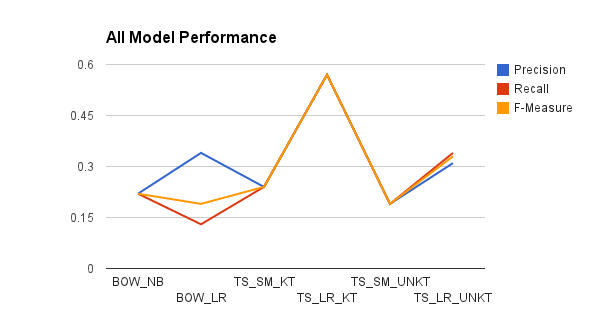
\includegraphics[width=\columnwidth]{allPerformance}}
\caption{All model performance using different metrics.}
\label{all-performance}
\end{center}
\vskip -0.2in
\end{figure} 


As we can see from Figure~\ref{all-performance}, we can see that the time series based model gives us way more better performance than content based model (TS is much better than BOW). The reason might be tweets content can only provide little information about the trend of the underlying topic they talk about. Or we haven't found a better way to use the content data.

Besides, Logistic Regression (LR) classifier works better than Naive Bayes (NB) classifier in content based Bag-of-Word model. This is not surprising that LR works better than NB, since NB assume the oder of words does't not matter, namely independence among a sequence of words. 


\subsection{Known vs Unknown Trend}

As shown in Figure~\ref{all-performance}, we can run our classification algorithm on both previous known trend (tested on 128 hours time series and regard the interval around peak as most salient trend) and unknown trend (tested on 8 months time series and detected most salient trend by our detection algorithm). We can see from the figure below that the Precision, Recall and F-measure became worse when we switch to use our own trend detection algorithm. 

This indicates that with a better trend detection algorithm, we can use the real time streaming data to predict a trend and a future hottest emerging trending pattern to a specific hashtag/topic. 


\section{Conclusion} 
We have introduced a method to do trend type cluster in the presence of large amounts of twitter data. With the detected pattern, we have derived twitter trend classification method based on temporal information. We also derived twitter trend pattern prediction method by applying naive bayes, similarity measurement and logistic regression method together with content and temporal information.

Given the result of experiment, we found that tweet content has a big connection with tweet trend patterns. But the key information for this is difficult to extract.  However, temporal information is a more direct representation of tweet trend and the time interval prior to a trend is a good indicator of future pattern of trend. 




% In the unusual situation where you want a paper to appear in the
% references without citing it in the main text, use \nocite
\nocite{langley00}

\bibliography{example_paper}
\bibliographystyle{icml2013}

\end{document} 


% This document was modified from the file originally made available by
% Pat Langley and Andrea Danyluk for ICML-2K. This version was
% created by Lise Getoor and Tobias Scheffer, it was slightly modified  
% from the 2010 version by Thorsten Joachims & Johannes Fuernkranz, 
% slightly modified from the 2009 version by Kiri Wagstaff and 
% Sam Roweis's 2008 version, which is slightly modified from 
% Prasad Tadepalli's 2007 version which is a lightly 
% changed version of the previous year's version by Andrew Moore, 
% which was in turn edited from those of Kristian Kersting and 
% Codrina Lauth. Alex Smola contributed to the algorithmic style files.  
